\documentclass[10pt]{PhDthesisPSnPDF}%
\usepackage{thesis_body}
\usepackage{pdfpages}
%%%%%%%%%%%%%%%%%%%%%%%%%

\usepackage{amsmath}%
\usepackage{amstext}%
\usepackage{amsfonts}%
\usepackage{amssymb}%
\usepackage{graphicx}
%\usepackage[latin1]{inputenc} 
\usepackage[T1]{fontenc}
\usepackage{authblk}
%\usepackage[bottom]{footmisc}
%\usepackage[top=3cm,left=2cm,right=2cm,bottom=2.5cm]{geometry} 
\usepackage[parfill]{parskip}
%\usepackage{titlesec}

%------------------------------------------------------------------
\hfuzz5pt % Don't bother to report overfull boxes < 5pt
\newtheorem{theorem}{Theorem} 
\newtheorem{corollary}[theorem]{Corollary}
\newtheorem{definition}[theorem]{Definition}
\newtheorem{example}[theorem]{Example}
\newtheorem{exercise}[theorem]{Exercise}
\newtheorem{lemma}[theorem]{Lemma}
\newtheorem{proposition}[theorem]{Proposition}
\pagestyle{plain}
%%% --------------------------------------------------------------
\DeclareGraphicsExtensions{.jpg,.pdf,.mps,.png}

%\setcounter{tocdepth}{6}
%\setcounter{secnumdepth}{6}
%\setcounter{chapter}{1}

\title{\Huge{An introduction to \\ applied data science} \\ 
\rule{100mm}{5pt} \\
\Large{A 5-day workshop towards practical \\ big-data applications and analytics}}
%  with practical experience extracting value from big data
\author{\Large{Eduardo Barbaro}}
\author{\Large{Coen Jonker}}
\affil{\normalsize Data Scientistists at Mobiquity Inc}
\date{\today}

% ----------------------------------------------------------------------
% turn of those nasty overfull and underfull hboxes
\hbadness=10000
\hfuzz=50pt


%%%%%%%%%%%%%%%%%%%%%%%%%%%%%%%%%%%%%%%%%%%%%%%%%
% Start-up
%%%%%%%%%%%%%%%%%%%%%%%%%%%%%%%%%%%%%%%%%%%%%%%%%
\begin{document}

\renewcommand\baselinestretch{1}
\baselineskip=14pt plus1pt

\pagenumbering{roman}    %  roman numbering for all preamble pages
\maketitle

% ----------------------------------------------------------------

\noindent{\textbf{About the workshop and this manual:}} \\

Welcome to ``An introduction to applied data science'' a 5-day original workshop thought and written by Eduardo Barbaro and Coen Jonker. At the end of this week you will be able to (i) understand the basics of data science, (ii) mathematically describe data, and (iii) munge\footnote{describes the constructive operation of tying together systems and interfaces that were not specifically designed to interoperate} it into an easy and communicable form. As the course develops, we will teach you how to access and look at data in innovative ways, as well as to extract value from big data. We aim a significant part of this training to help you create and interpret a diverse set of numerical models, as well as to calculate descriptive analytics while fully understanding their meaning. We also focus on presentation, and how to show your results in beautiful smart charts and tables.

Although all the computations will be performed in Mobiquity's AWS cloud, we will guide you through all the necessary steps to install any software necessary for this course in your local machines. We use Mobiquity's AWS cloud to get the benefit of running our code in a fast, secure, and controlled environment.

This manual is divided in 11 independent short chapters. In Chapter \ref{DS} we set the stage with a short introduction to then answer together a bold question: ``what is data science?''. In Chapter \ref{basics} we will spend some time to recap some basic mathematical concepts needed throughout the entire workshop. Chapters \ref{P1} and \ref{P2} are devoted to (important) practicalities, such as installing software/libraries and getting familiar with the AWS cloud environment. We also teach you some basic programming skills, so we are all on the same page. We move forward to our first data harvest, in Chapter \ref{harvesting}. We teach you how to manipulate data, as well as to properly describe and clean it. Chapter \ref{numerics} covers the basics of designing a smart numerical experiment. 

Chapters \ref{MLearn} to \ref{bigData} cover more advanced topics such as machine learning tools, databases (SQL and no-SQL) as well as a mapreduce implementation (Hadoop). In particular, in Chapter \ref{bigData} we show in detail how to load, transform, and extract value from real big data. Finally, in Chapter \ref{Commun} we come back to basics to show you rudiments of plotting and how to communicate your results. 

We wish you a pleasant learning!

\newpage
\thispagestyle{empty}
\mbox{}
\cleardoublepage

% Counting	
%\setcounter{page}{1}
\setcounter{tocdepth}{2}


%%%%%%%%%%%%%%%%%%%%%%%%%%%%%%%%%%%%%%%%%%%%%%%%%
% Table of contents
%%%%%%%%%%%%%%%%%%%%%%%%%%%%%%%%%%%%%%%%%%%%%%%%%

%{\baselineskip=.8\baselineskip % shortens the spacing between lines in the TOC

\setcounter{secnumdepth}{3} % organisational level that receives a numbers
\setcounter{tocdepth}{2}    % print table of contents for level 3
\tableofcontents            % print the table of contents


%%%%%%%%%%%%%%%%%%%%%%%%%%%%%%%%%%%%%%%%%%%%%%%%%
% List of Figures and Tables
%%%%%%%%%%%%%%%%%%%%%%%%%%%%%%%%%%%%%%%%%%%%%%%%%
	
%\addcontentsline{toc}{chapter}{List of Figures}
%\listoffigures 
%\cleardoublepage
%\addcontentsline{toc}{chapter}{List of Tables}
%\listoftables 
%\cleardoublepage

%%%%%%%%%%%%%%%%%%%%%%%%%%%%%%%%%%%%%%%%%%%%%%%%%
% Chapters 
%%%%%%%%%%%%%%%%%%%%%%%%%%%%%%%%%%%%%%%%%%%%%%%%%

\cleardoublepage
% Introduction
\newpage
\pagenumbering{arabic}	 %  arabic numbering for all preamble pages


\chapter{A historical view on data science}\label{DS} 

In this Chapter we briefly try to shed some light on the question ``what is data science?''. First of all, it is important to realize that data science is not a new concept. There are many complex definitions out there, but in our view, data science is simply the coupling of very well-established disciplines, such as mathematics and statistics, with a relatively young discipline, computer sciences. 

Have a look at Fig. \ref{fig:Analytics}. It shows the evolution of 5 fundamental disciplines related to data science (Mathematics, Statistics, visualization, technology, computer science). Note that this cartoon depicts events as old as the ``invention'' of modern calculus by Newton/Leibniz (in the 17$^{th}$ century) or foundation of probability theory by Cardano (in the 16$^{th}$ century). You can see that back in those times all the disciplines were really self-contained areas without much interconnection. As we enter the 20$^{th}$ century things start to get more interconnected. Statistics and Mathematics cannot be separated so clearly any more (e.g. stochastic models, survival models), and computer sciences and technology started to gain more terrain (e.g. relational databases, tree-based models). 
\newpage
\begin{figure}[h]
	\begin{center}
			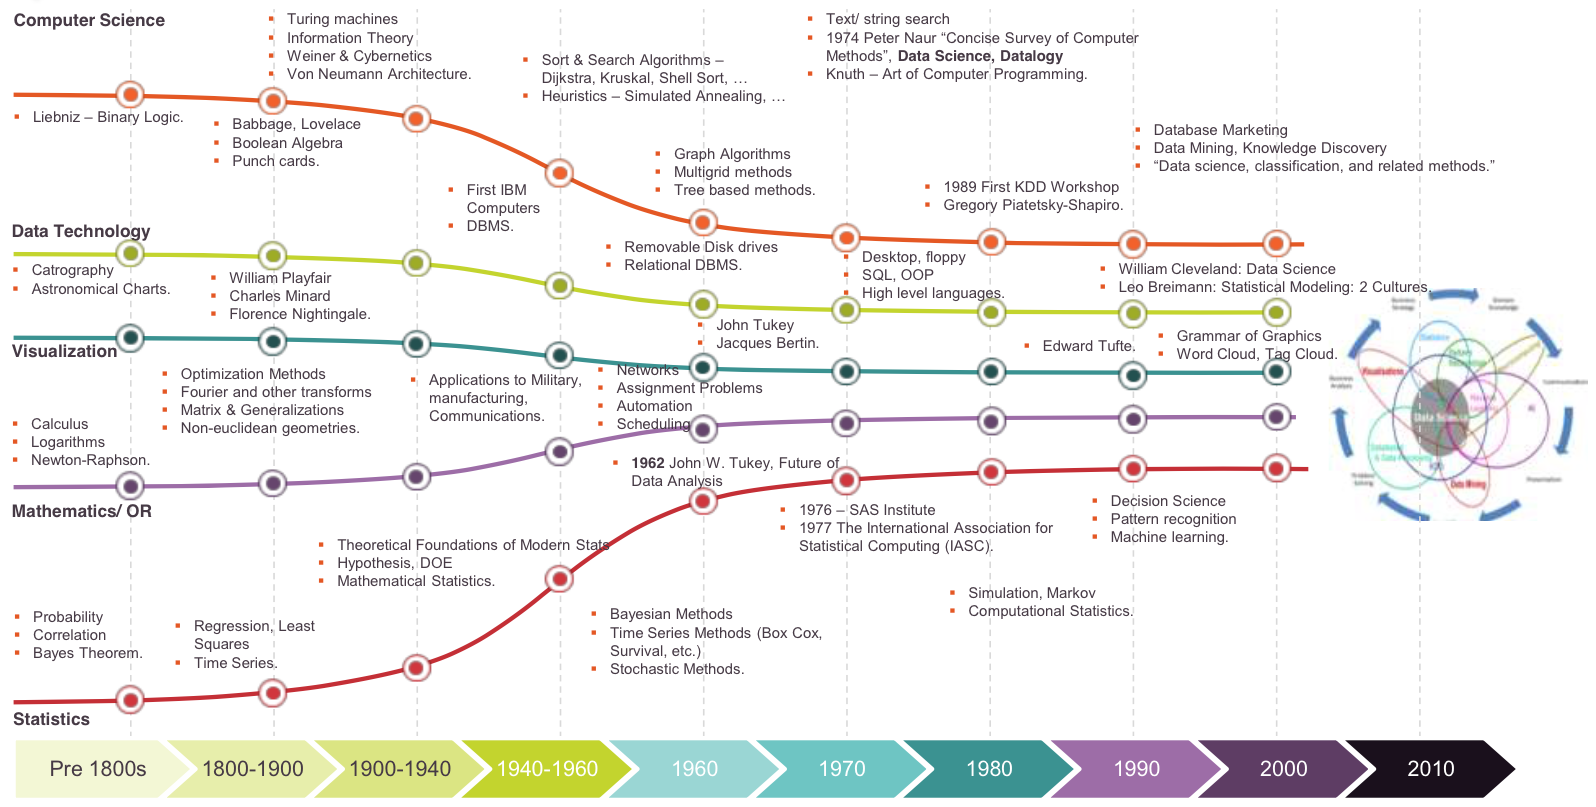
\includegraphics[scale=0.25]{HistoryCH1}
	\end{center}
	\caption{Most important events in the history of data science. \textit{Credit: Mamatha Upadhyaya}}
	\label{fig:Analytics}
\end{figure} 

As early as 1962, John Wilder Tukey, an American Mathematician, wrote in his ``The future of data'':
\begin{quotation}
\textit{For a long time I thought I was a statistician, interested in inferences from the particular to the general. But as I have watched mathematical statistics evolve, I have had cause to wonder and doubt. I have come to feel that my central interest is in data analysis. Data analysis, and the parts of statistics which adhere to it, must take on the characteristics of science rather than those of mathematics data analysis is intrinsically an empirical science.}
\end{quotation} 
 
That served as inspiration to Tukey who, in 1977, published his most well-known book ``Exploratory Data Analysis''. In that book, he argued that exploratory and confirmatory data analyses must proceed alongside. Also in the 1970's, Peter Naur, Danish computer science pioneer, published the important ``Concise Survey of Computer Methods''. In this book, the term data science was used for the first time. According to him, data science can be defined as:
\begin{quotation}
\textit{The science of dealing with data, once they have been established, while the relation of the data to what they represent is delegated to other fields and sciences.}
\end{quotation} 

In the beginning of the 21$^{st}$ century all the disciplines related to data science merged. In 2008, Jeff Hammerbacher (Facebook) and DJ Patil (LinkedIn) used the terminology ``Data scientist'' to define their work and teams. Since then, the use of this terminology has fully infiltrated the vernacular, and did not stop growing. 

Today, data science and computer sciences (through machine learning) have been put together as almost synonyms. There are new terminologies appearing every year, such as Deep Learning, Big Data, Data Mining. Today, we understand that data science and big data do not mean (just) ``lots of data''. Instead, it means the creation of a new paradigm in how we do analysis and combine the use of our traditional tools (Mathematics and Statistics) with the technology available nowadays.

\chapter{Some basics and beyond}\label{basics}

Before we start with some hands-on data science, we think it is fundamental to ensure we are all on the same page on the Mathematics and Statistics we need throughout this course. But don't worry, it is nothing fancy. We, by no means, have the intent to \textit{formally} teach you any Mathematics. Instead, we just want to refresh some of the concepts we already know, but may have forgotten throughout the years.

\section{Mean, median, and standard deviation}

We would like to start with a good look at Fig. \ref{fig:boxplot}. This type of graphical representation is called a box-plot\footnote{The box-plot was created by John Wilder Tukey, the American Mathematician we talked about in Chapter 1.}. It shows the variation in miles per gallon (MPG) for cars with different numbers of cylinders\footnote{This data was extracted from the 1974 Motor Trend US magazine}. For now, let's focus only on cars with 4 cylinders. The black line just above 25 MPG is called median, i.e. the middle of the dataset. It indicates the point such that there is an equal probability of a MPG value falling above or below it. The top/bottom edges of the box indicate the upper and lower quartile, respectively. These quartiles tell us that there is only 25$\%$ chance a car with 4 cylinders will use more than 30 or less than 23 MPG. \textit{Did you realize that already 50$\%$ of our data lies within the box?} The horizontal lines above/below the box represent the maximum/minimum MPG values excluding outliers. Here, outliers are defined as MPG which appear less often than 10$\%$ of the cars with 4 cylinders, i.e. above 34 MPG or below 21 MPG.

\begin{figure}[h]
	\begin{center}
			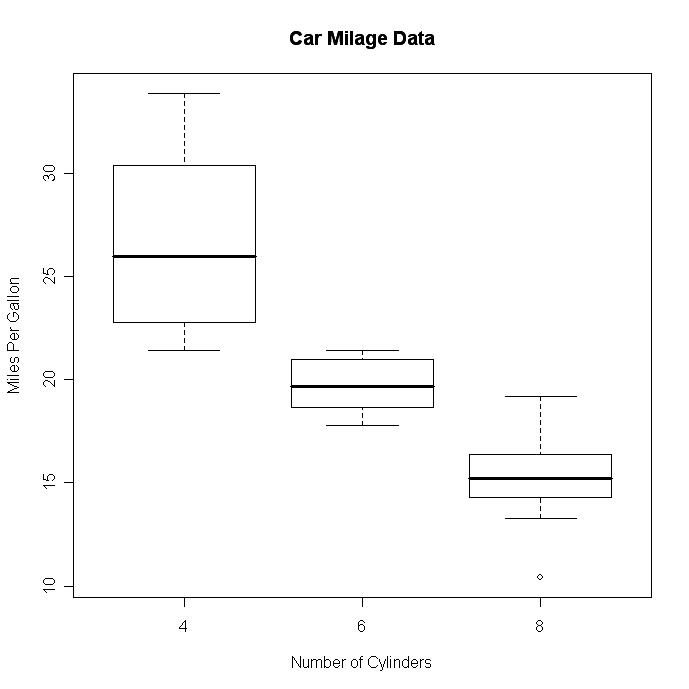
\includegraphics[scale=0.3]{milleagech2}
	\end{center}
	\caption{Box-plot of miles per gallon by car cylinders. This data was extracted from the 1974 Motor Trend US magazine.}
	\label{fig:boxplot}
\end{figure} 

Note that the thick horizontal black lines inside the boxes represent the respective \textit{medians} for 4, 6 or 8 cylinders. Note that this value is different than the mean value. Here is why: the ``mean'' represents the ``average'' we all know. Simply sum up all the numbers and then divide them by the total number of occurrences. The ``median'' represents the ``middle'' of a ordered series of numbers. This is important because in practice we always find distributions which are highly skewed. In those cases, the median is more representative than the mean.

The mean or the median alone do not tell us the whole story about our data. We still have to understand the data \textit{distribution} and how the individual points are spread around the mean. To help us with that we will introduce the concept of standard deviation. In a nutshell, it represents by how much the individual samples differ from the mean. We depict it in Fig. \ref{fig:std}.

\begin{figure}[h]
	\begin{center}
			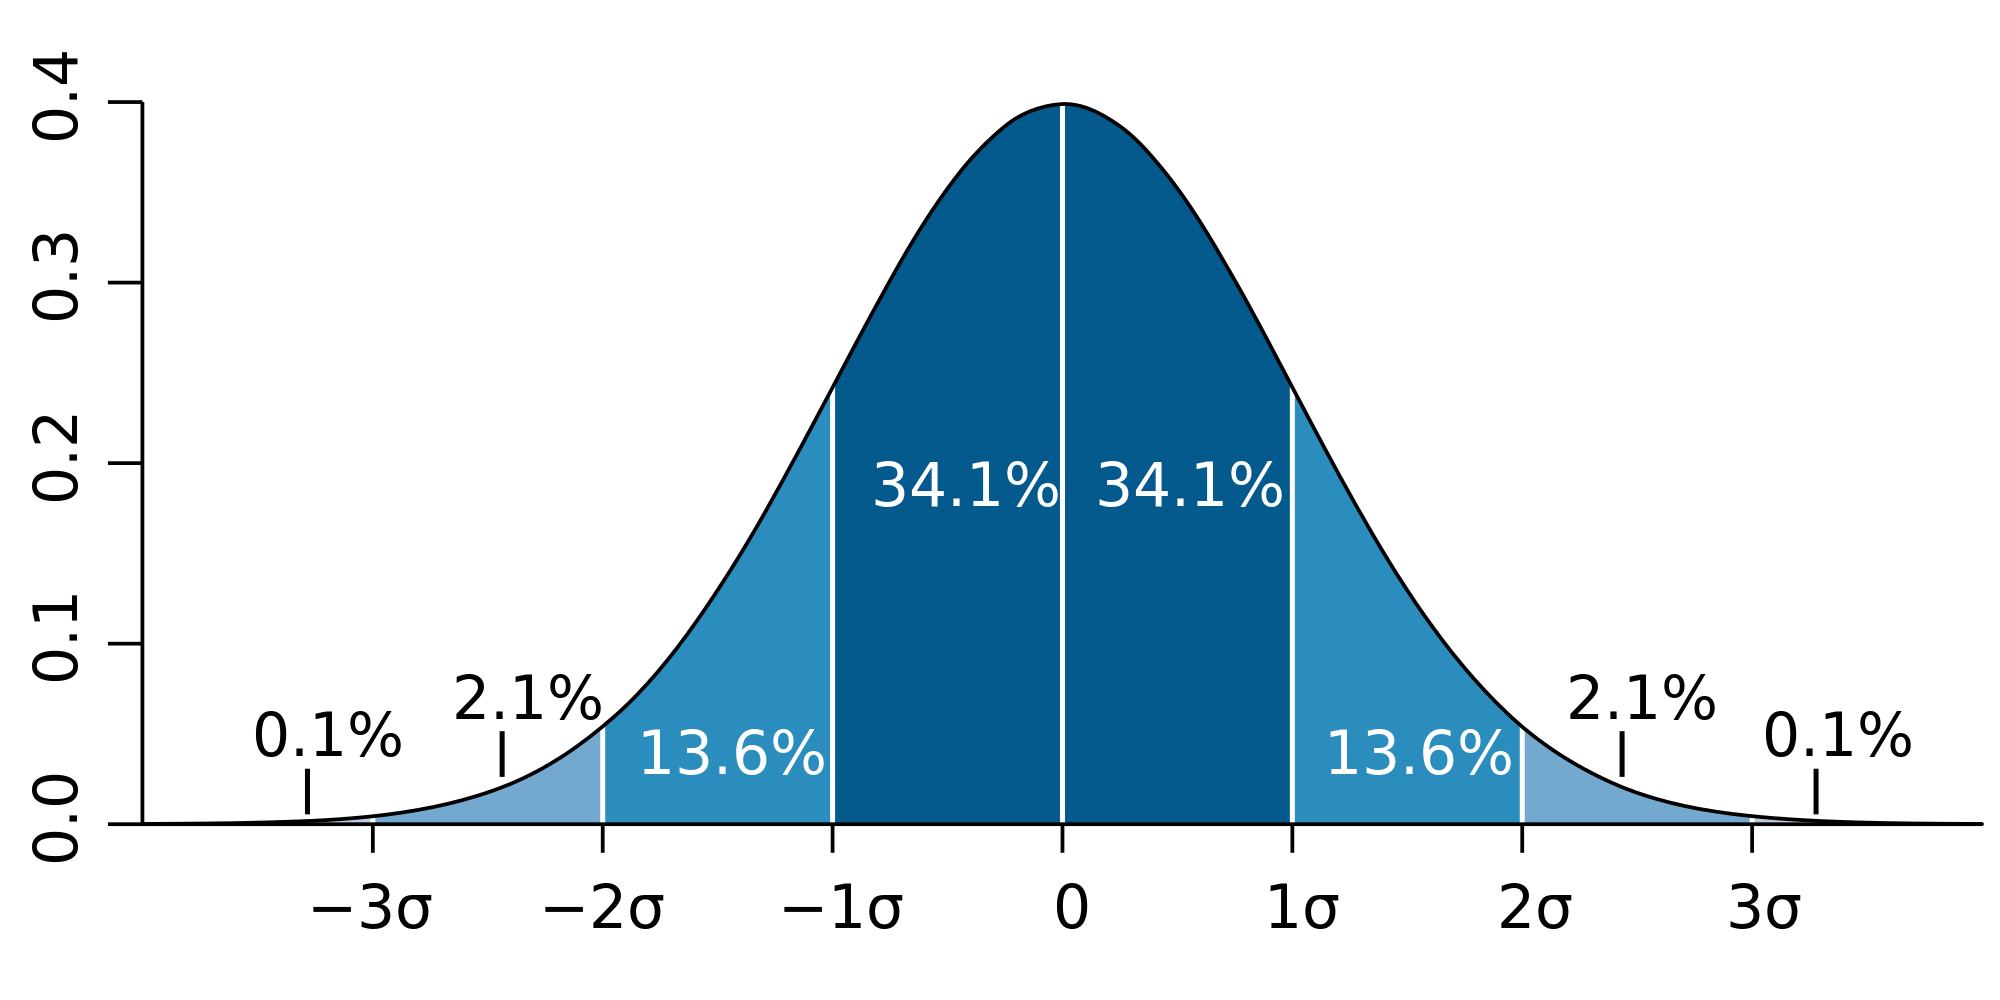
\includegraphics[scale=0.13]{stdch2}
	\end{center}
	\caption{Normal distribution where each band accounts for $\pm$ 1 standard deviation}
	\label{fig:std}
\end{figure} 

\newpage

The standard deviation is a measure of the dispersion of your data. That means a small standard deviation indicates little dispersion around the average. In contrast, a high standard deviation indicates significant dispersion around the average. As shown in Fig. \ref{fig:std}, the width of one standard deviation ``covers'' roughly 68$\%$ of the data dispersion. That number increases to 99$\%$ for three standard deviations.

\section{Interpreting a plot, tracing a linear fit, and understanding R$^2$}

Another important topic we want to talk is how to interpret plots. As we show in Chapter \ref{Commun} plots are a fundamental way to communicate your data-science results within your company. For now, we will focus on extracting some interesting information from Fig. \ref{fig:linR}. Later, we go in much greater detail on how to design and interpret such results.

\begin{figure}[h]
	\begin{center}
			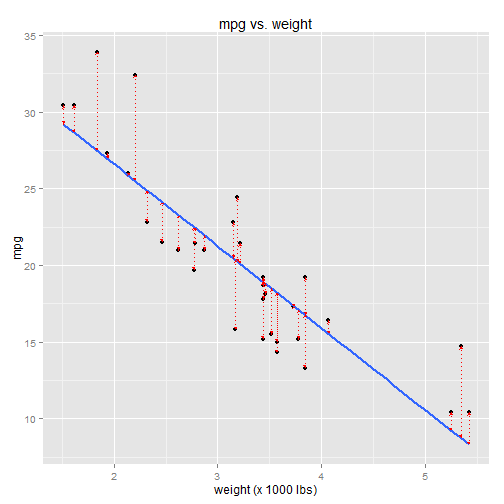
\includegraphics[scale=0.35]{linregch2}
	\end{center}
	\caption{Miles per gallon versus the weight of the cars. The blue line draws a linear relation between MPG and the weight of the cars. The red dotted-lines represent the difference (residuum) between the linear fit and each data point. This data was extracted from the 1974 Motor Trend US magazine.}
	\label{fig:linR}
\end{figure} 

We observe a negative correlation between MPG and weight of the car. As the weight increases, MPG decreases. Note that this follows intuitively, since we expect heavier cars to use more fuel and therefore have lower MPG. The blue line represents a linear fit between the variables. The criterion to obtain the linear fit is to minimize the distance between the fit and the data points. This difference is called residuum (shown in red in Fig. \ref{fig:linR}). In Chapter \ref{numerics} we will cover the design of such simple numerical model in great detail. 

\newpage

For now let's assume we know how to implement such model - but how do we measure its performance? A simple way to achieve that is by calculating the so-called \textit{determination coefficient}, more known as (R$^2$). R$^2$ is a metric that uses the residua information to determine if a linear fit is acceptable or not. It ranges from 0 to 1, where zero means no correlation between variables and 1 means a perfect fit. In the case shown in Fig. \ref{fig:linR} we find that $R^2=0.75$, indicating a good linear fit between MPG and weight of the car. In other words, the weight of the car can explain 75$\%$ of the MPG's variance. Generally speaking we define $R^2>0.5$ as acceptable. The 

\section{Histograms}

The last topic we want to cover in this Chapter is histograms. A histogram is nothing more than a plot consisting of bars whose area represents the frequency of a given variable. In Fig. \ref{fig:histch2} we can visualize a histogram showing the frequency of the MPG variable:

\begin{figure}[h]
	\begin{center}
			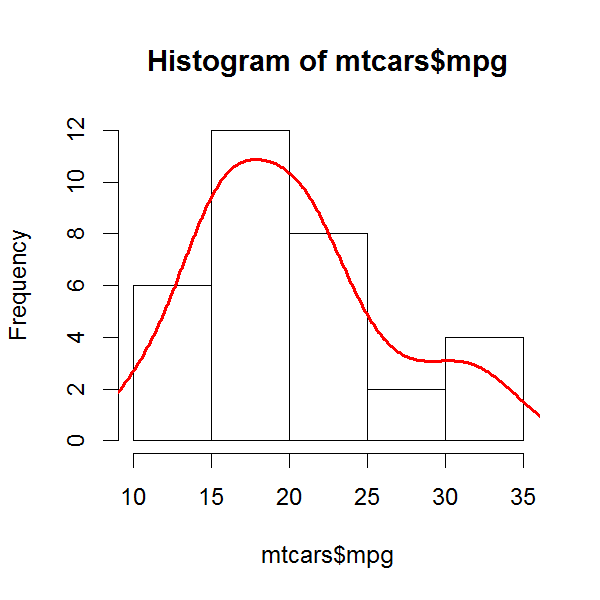
\includegraphics[scale=0.7]{histch2}
	\end{center}
	\caption{Histogram showing the MPG frequency distribution. This data was extracted from the 1974 Motor Trend US magazine.}
	\label{fig:histch2}
\end{figure} 

\newpage

Note that the width of the bars represents the class interval. In our case every bar shows the frequency for an interval equal to 5 MPG. We can conclude from this plot that most cars have a MPG usage between 15 and 20. This plot also triggers many more questions, such as why is the frequency of cars using 30-35 MPG higher if compared to 25-30 MPG? In order to answer this type of questions our strategy is to combine a number of plots and understand the variables behaviour. We will demonstrate that in the next Chapters.

\chapter{Practicalities: Software Installations and AWS cloud}\label{P1}
\chapter{Practicalities: Programming language and libraries}\label{P2}
\chapter{Harvesting data}\label{harvesting}
\section{Data Manipulation}\label{dataM} 
\section{Analytics 1: Describing your data}\label{Analy.1}
\section{Analytics 2: Cleaning your data}\label{Analy.2}
\chapter{Numerical Modeling}\label{numerics}
\section{Basics}\label{numBasics}
\section{Designing smart numerical experiments}\label{NumDesign}
\chapter{Machine learning tools}\label{MLearn}
\section{Supervised methods}
\section{unsupervised methods}
\chapter{Databases}\label{databases}
\section{SQL}
\section{NoSQL}
\subsection{MongoDB}
\chapter{Map Reduce}\label{mapR}
\section{Hadoop}
\chapter{Big Data}\label{bigData}
\chapter{Communicating Results}\label{Commun}
\section{Visuals}\label{Visuals}

%supervised learning (trees and forests, nearest neighbor, regression)
%optimization (gradient descent)
%unsupervised learning (clustering, )





%http://work.caltech.edu/telecourse


%\begin{equation}
%T=\frac{1}{2}\cdot \sum{(X_i - X_{i-1})\cdot(Y_i+Y_{i-1})}
%\label{eq:T}
%\end{equation}
%
%\
%   
%
%\begin{figure}[h]
%
%	\begin{center}
%		$\begin{array}{c@{\hspace{1in}}c}
%%			\includegraphics[scale=0.25]{Simpsons} &
%%			\includegraphics[scale=0.45]{Simpson} \\ [0.4cm]
%			\mbox{\bf (Homer Simpson)} & \mbox{\bf (Metodo de Simpson)}
%		\end{array}$
%	\end{center}
%	\caption{Metodo de Simpson}
%	\label{fig:Simpson}
%\end{figure}
%
%\pagebreak
%
%
%\begin{eqnarray}
%S=1474379,23\;pes^2  \nonumber \\
%S=33,85 \;acres
%\label{eq:}
%\end{eqnarray}

\end{document}